\documentclass[10pt,conference]{IEEEtran}

\usepackage[utf8]{inputenc}
\usepackage{eurosym}
\usepackage{graphicx} 
\usepackage{hyperref} 
\usepackage{amsmath}

\title{Final Project CS:Video Game Head Soccer }

\author{%
    \IEEEauthorblockN{Sebastian Emilio Moscoso Riveros}
    \IEEEauthorblockA{%
      E.P. Ciencia de la Computación\\
      Univesidad Católica San Pablo\\
      Arequipa, Perú\\
      Email: \href{mailto:sebastian.moscoso@ucsp.edu.pe}{\textbf{sebastian.moscoso@ucsp.edu.pe}}}
    }

\begin{document}
    
\maketitle

\begin{abstract}
    This project is a video game based on  OOP .\\
    For this project , I worked in c++ with openGL.So I will explain the process of the creation of this video game.
\end{abstract}

\section{Introduction}
    The first part in the project was ,chosen the type of video game that I want . So I chose Head Soccer , because I love play soccer.The second part was , chosen the part of  graphics to development the video game and the design pattern ;I chosen  openGL because it has the perfect  toolkit to develop my video game , and my design pattern  is Mediator Design Pattern.
\section{Learning Part }
    This was the part most important to develop the game,that
    was learned openGL , because it have the toolkit to do my
    game, so for me , is important that in the learning process the person develop the game with the basic knowledge , that is gain every time that proof some new.\\
    So for learning the most basic was :\\
    1.Library linker\\
    2.Create a Window\\\
    3.Shaders\\
    4.Textures\\
    5.Transformations\\
    
\begin{figure}[h!]
\centering
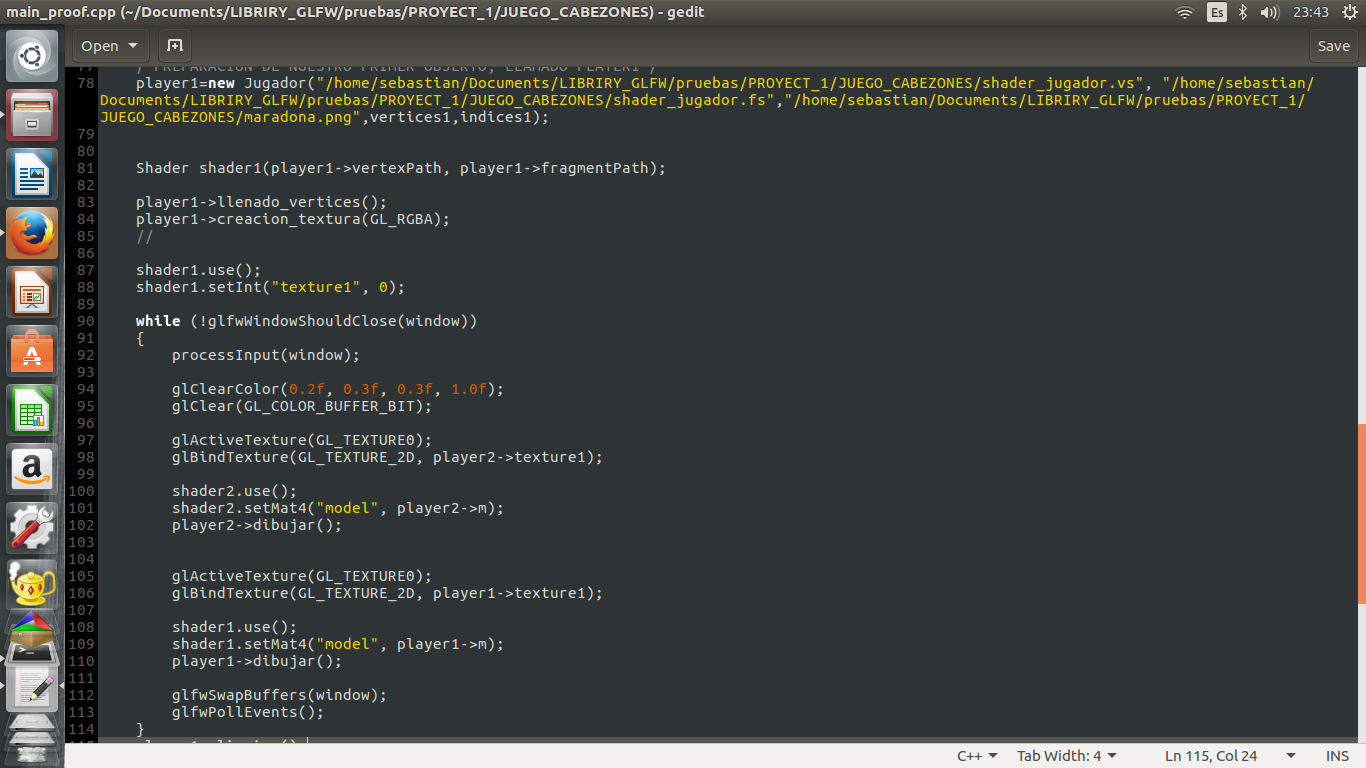
\includegraphics[scale=0.15]{code_imagen.png}
\caption{Part of code ,loading a image }
\label{fig:code}
\end{figure}

\section{Develop of the first part}
    The first part ,I started with the development of  examples
    ,learning the topics that I needed to develop the structure of my game .
\begin{figure}[h!]
\centering
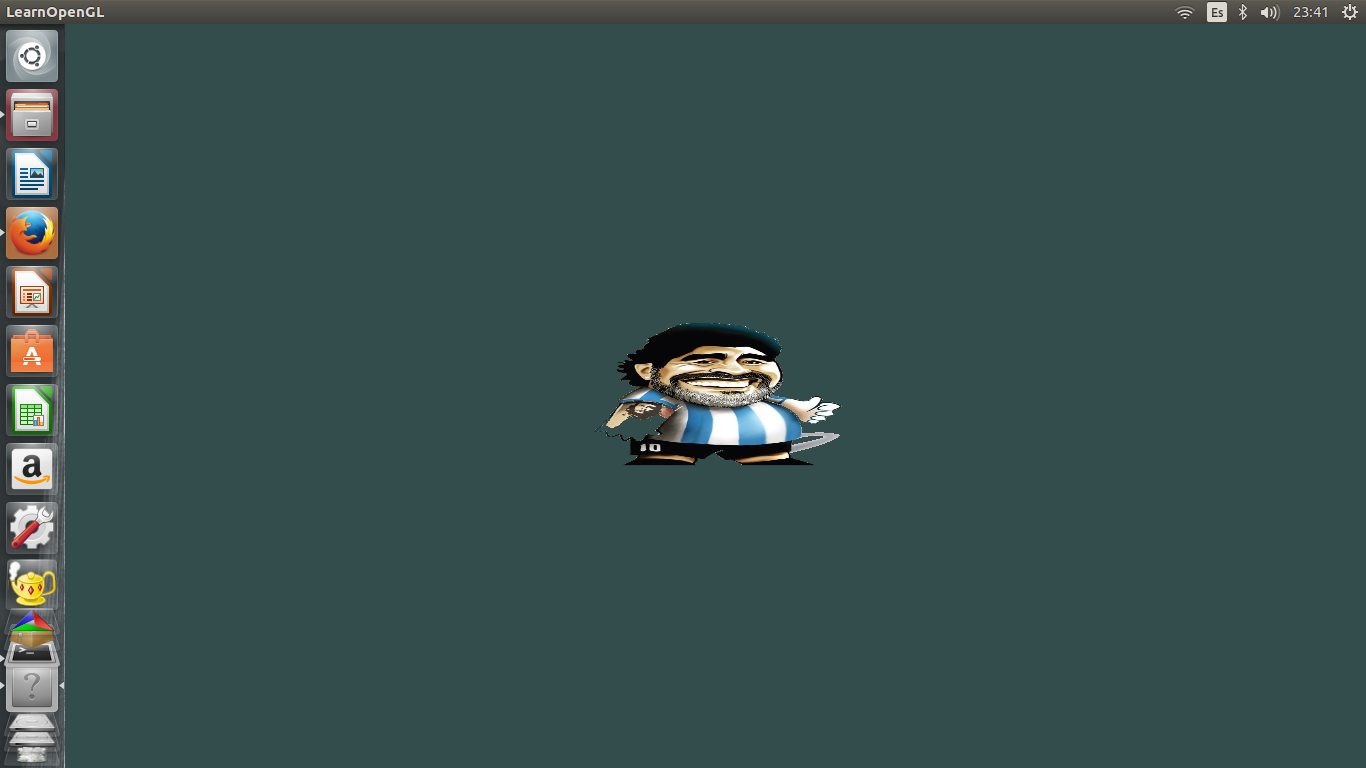
\includegraphics[scale=0.14]{implementacion.png}
\caption{  Image that was develop like a first object in the scene }
\label{fig:Object player}
\end{figure}
    
\section{Develop of the second part}
    The second part ,I started with the development of classes in my game ,in  separate parts;the joined all in a main , i get a structure like this:
\begin{figure}[h!]
\centering
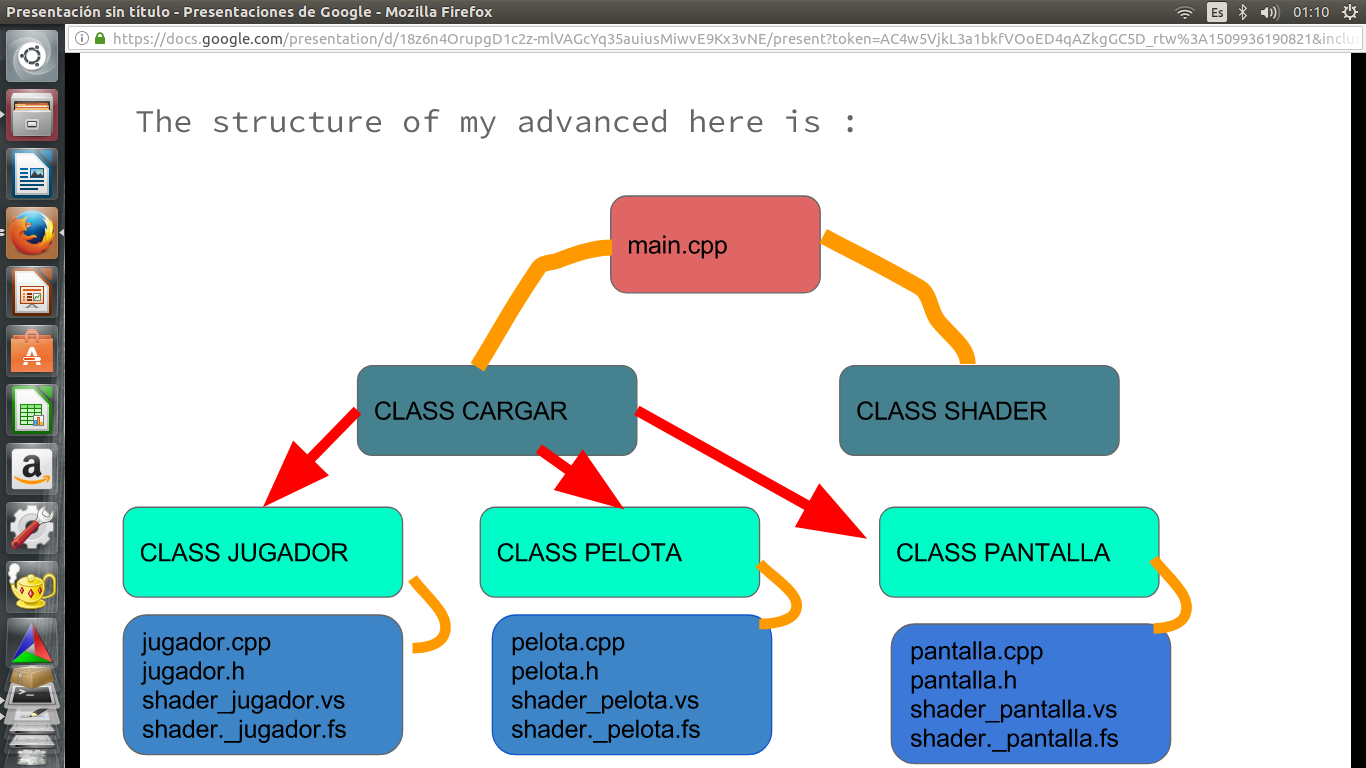
\includegraphics[scale=0.14]{estrucura.png}
\caption{  The first structure that I get in my code }
\label{fig:Strucutre1}
\end{figure}    
    This structure represent the part of develop all my objects in scene.
\begin{figure}[h!]
\centering
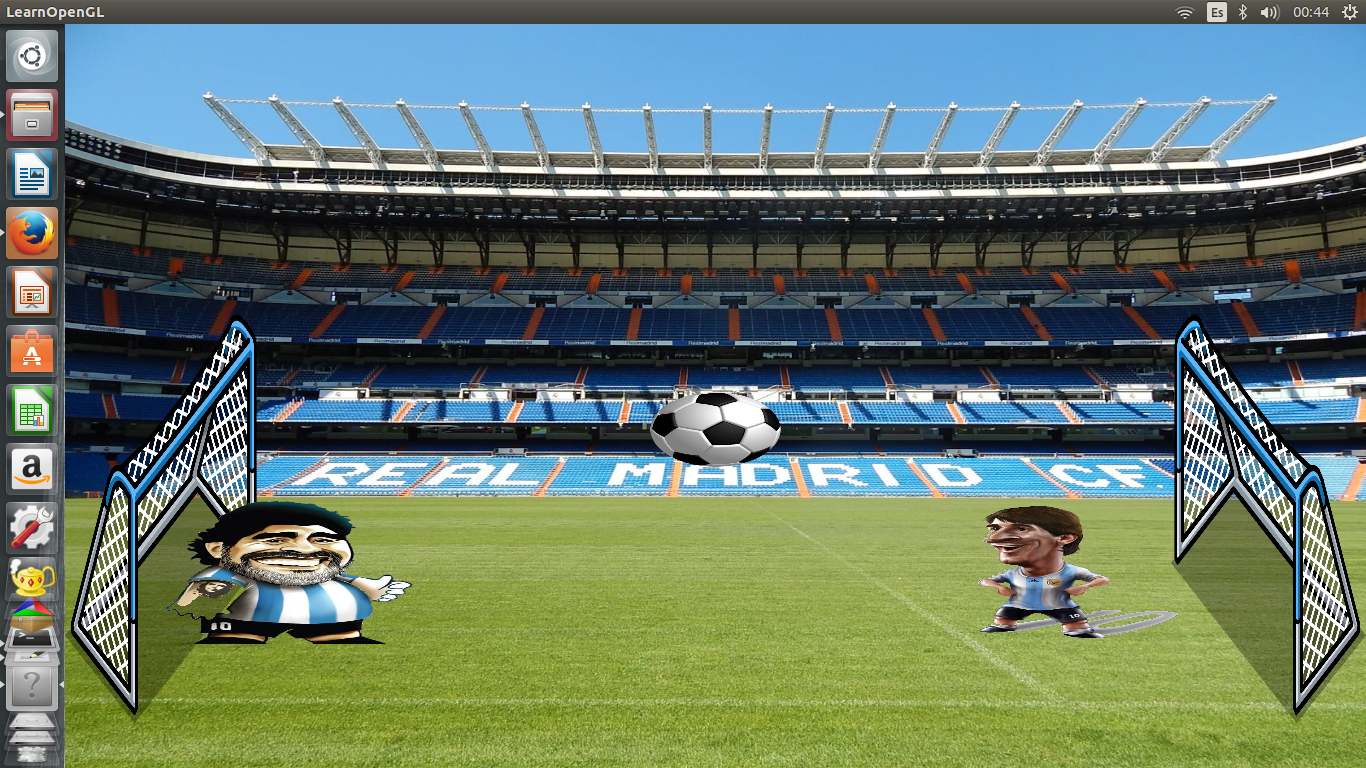
\includegraphics[scale=0.14]{avance.png}
\caption{  The first structure that I get in my code }
\label{fig:Struutre scene }
\end{figure}     
    
\end{document}
